\begin{abstract}
	On the MSc course "\textit{Computer Modelling Laboratory}" at ELTE, I have worked on a project in nuclear physics, where I studied the behaviour of the Japanese NEBULA detector when it was bombarded by neutron beams. For the simulation and analysis I've used the Geant4 general-purpose software, which is capable of producing state-of-the-art simulations and results in almost any field in nuclear- or particle physics.
\end{abstract}

\begin{multicols}{2}
\section{Introduction}
On the third regular meeting I have presented my plan to explore the different, built-in, so-called \q{physics list} in Geant4 and discover some of the differences between them in my neutron simulation. Besides working with the different physics list, I have also implemented a new data analysis method for my simulation pipeline.

\section{Particle tracking in Geant4}
Geant4 simulations can be divided into 3 different levels. The simulation will behave differently or store different informations on different levels. We can give these levels the names \q{step level}, the \q{event level} and the \q{run level}.

\subsection{Step level}
Simulations in Geant4 work just like almost any other computer simulations. The time is discretized and the simulation advances in smaller $dt$ long steps, updating the parameters and quantities constantly. This is why the bottom and highest resolution level of the Geant4 simulation is this step-wise stream of information.

This is the most (and only) versatile level in tracking quantities, which won't accumulate over time and/or would change value at basically every other step. Quantities like the polarization of a particle, its charge, the magnitude of the electric/magnetic field, the physical process happening in a simulation step, etc. are all step-dependent and can't be agglomerated.

\subsection{Event level}
An \q{event} in Geant4 is the set of all steps taken by a user-defined particle and all the steps the presence of the particle induced. What this means is, that when we shot a particle into a simulation and it happens to create a new particle through some arbitrary physical process, the software has to start to track the newly created particle too, through a series of simulation steps. These are appended to the set consisting of the steps of the original particle. These together form an event in Geant4.

Disadvantage of using the event level to track time evolution of quantities is that on this level we can easily handle only accumulative quantities, such as energies. We can analyse eg. how much energy a neutron lost during its lifetime by broadcasting deposited energy values from the step level and accumulating them on the event level, resulting in the total energy deposited during the full event.

\subsection{Run level}
The uppermost one is the \q{run level}, which encompasses every event in the simulation. The \texttt{UserRunAction} class is the direct operator of the particle generation and it conducts the simulation of the individual Geant4 events, as well it handles data I/O.

\section{Exploration of Geant4's \q{physics lists}}
The so-called \q{physics list} in Geant4 are collections of physical processes. They explicitly determine what physics Geant4 should utilize when running a simulation. They define different effects, different interactions, which lists can be customized at will to suit our simulation. Certain physical effects only relevant at lower energies, some only at higher energies. And if we don't choose appropriate physics for our simulation, it will be simply inaccurate. Of course different physics means different results, and that's why it is an important question to ask, what physical framework should be used in a novel simulation.
\begin{Figure}
	\centering
	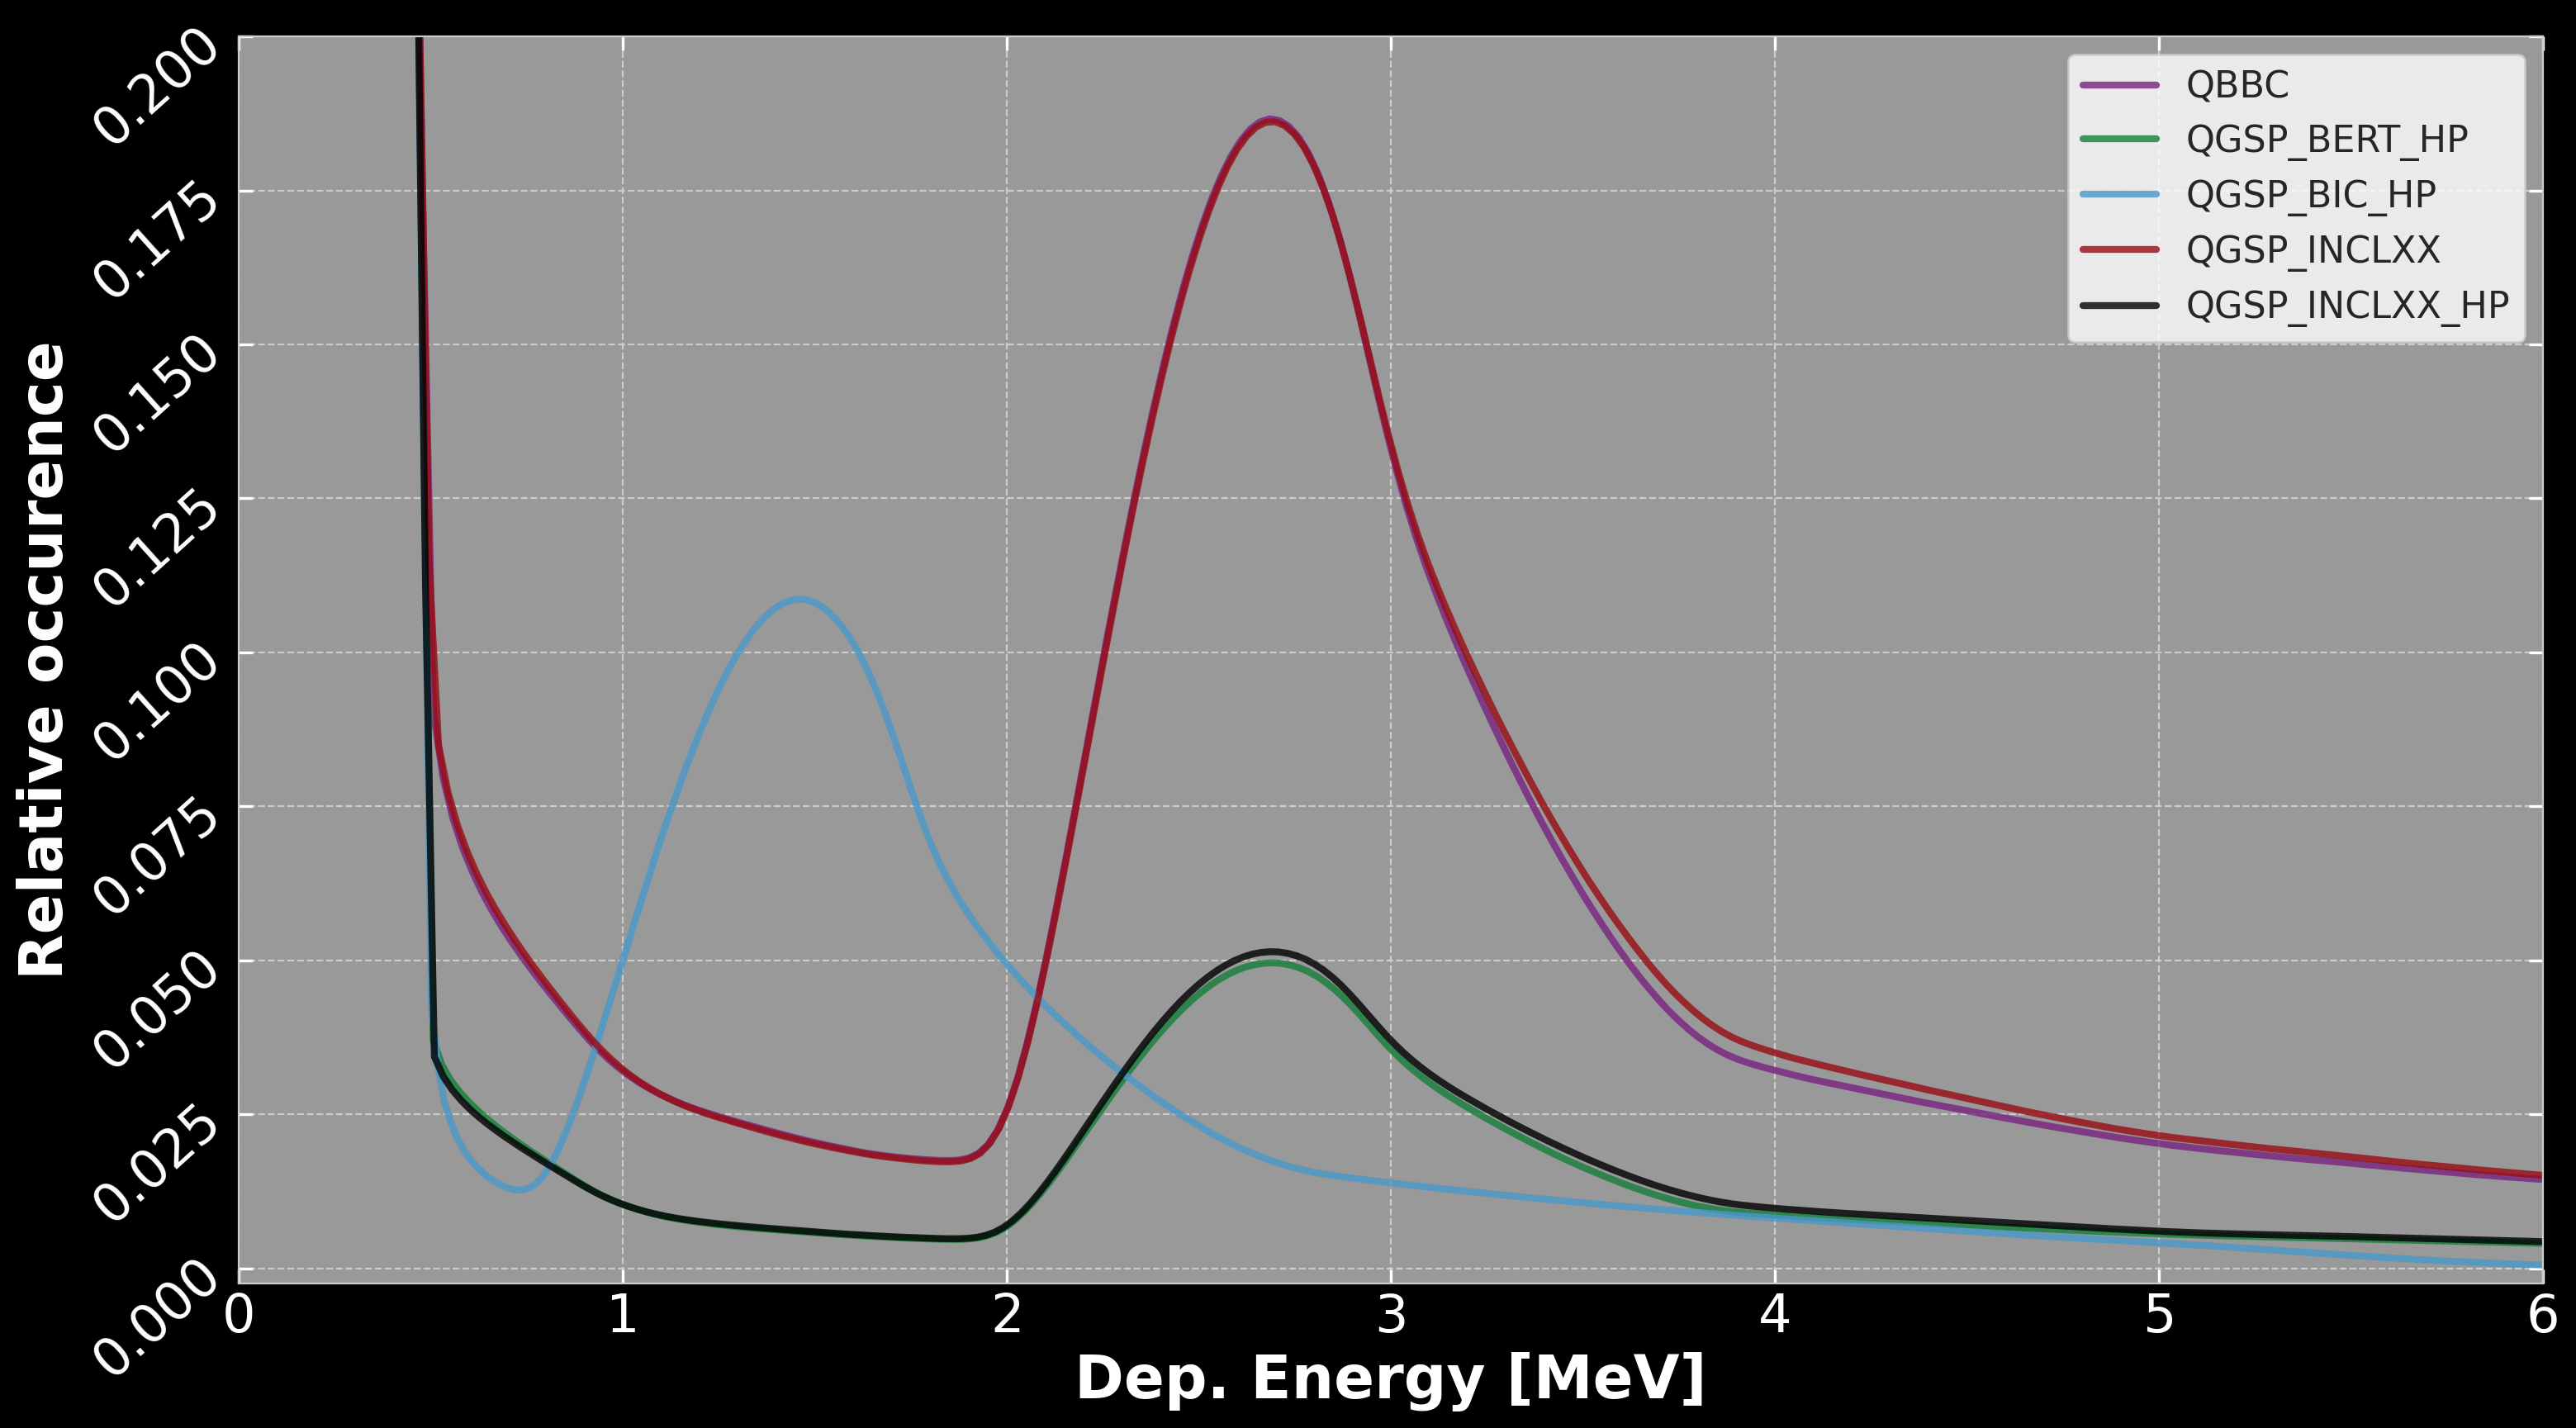
\includegraphics[width=\linewidth]{{images/energy_dist_full_concat_E100.png}}
	\captionof{figure}{} \label{fig:1}
\end{Figure}
On Fig. \ref{fig:1} we can see the difference of the KDE of energy deposit for different physics lists in Geant4. It can be seen that there are obviously big differences between different physics types. One can say, that for neutrons with smaller energies, the physics list ending with the \texttt{HP} tag in their names should be used, which contain the so-called \q{data driven high precision neutron} package.

\section{Explored quantities}
Besides the deposited energy I've also explored the occurence of physical processes in the simulation.  What you would see on this figure is that the three most frequent events are the energy deposit of hadron ionization (\texttt{hIoni}), the elastic collision of hadrons (\texttt{hadElastic}) and the energy deposit of electron ionization (\texttt{eIoni}). Of course if the physics list changes, the processes also change. Some processes are dropped, new processes are introduced, proportions are changing around. The difference between two different physics lists can be seen on Fig. \ref{fig:2} and Fig. \ref{fig:3}.

We can also plot the processes by their contribution to the total energy deposit. We can see, that for $100$ MeV in case of this simplified NEBULA detector, the hadron ionization deposited the most energy during the simulation, with ion ionization and electron ionization following it on the second and third places. This is so robust, that this distribution was the very same for other processes too. These quantities can be seen on Fig. \ref{fig:4} and \ref{fig:5}.

We can also explore the distribution of all the different particle steps during the simulation as seen on Fig. \ref{fig:6} and Fig. \ref{fig:7}.

\section{Plans for next week}
For the final lecture I'll plan to examine the detection efficiency of the NEBULA detector for different energy levels. This is an important measure of the detector and will serve as a good and important task to end the project with.
\end{multicols}

\newpage
\section{Appendix: Figures}
\subsection{Process distribution in two different physics lists}
\begin{figure}[h]
	\centering
	\captionsetup{font={normalsize}}
	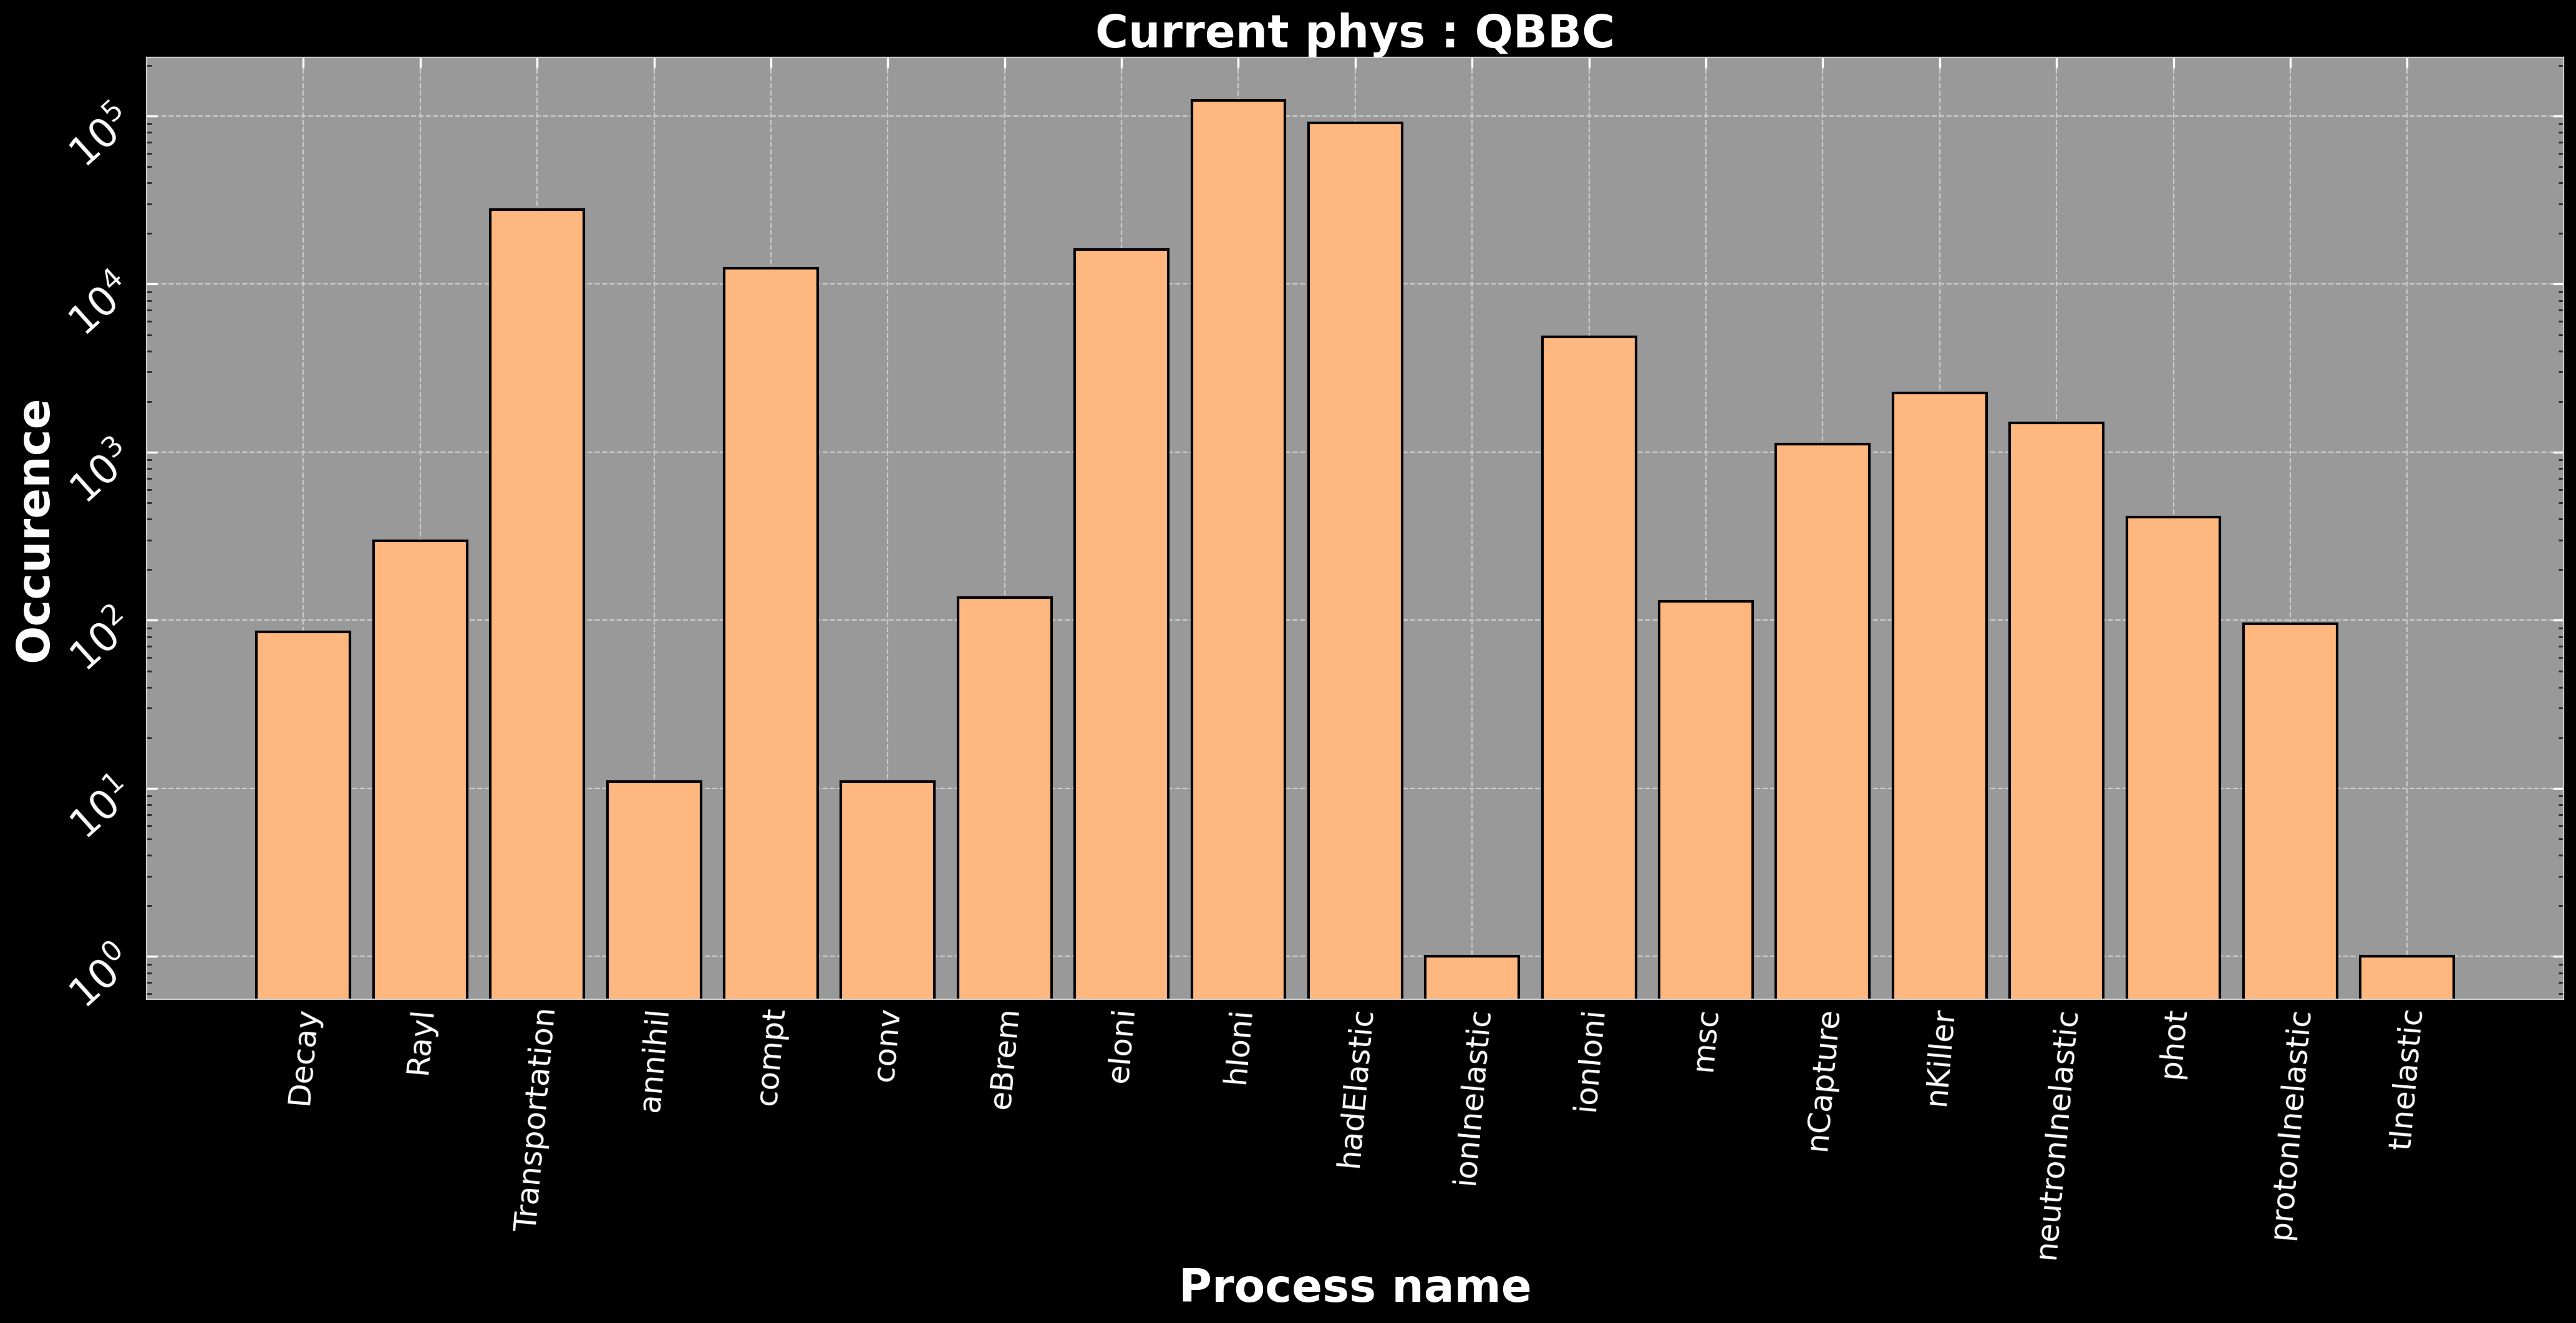
\includegraphics[width=0.95\textwidth]{{images/process_dist_E100_phQBBC.png}}
	\captionof{figure}{}\label{fig:2}
\end{figure}
\vspace{-5pt}
\begin{figure}[h]
	\centering
	\captionsetup{font={normalsize}}
	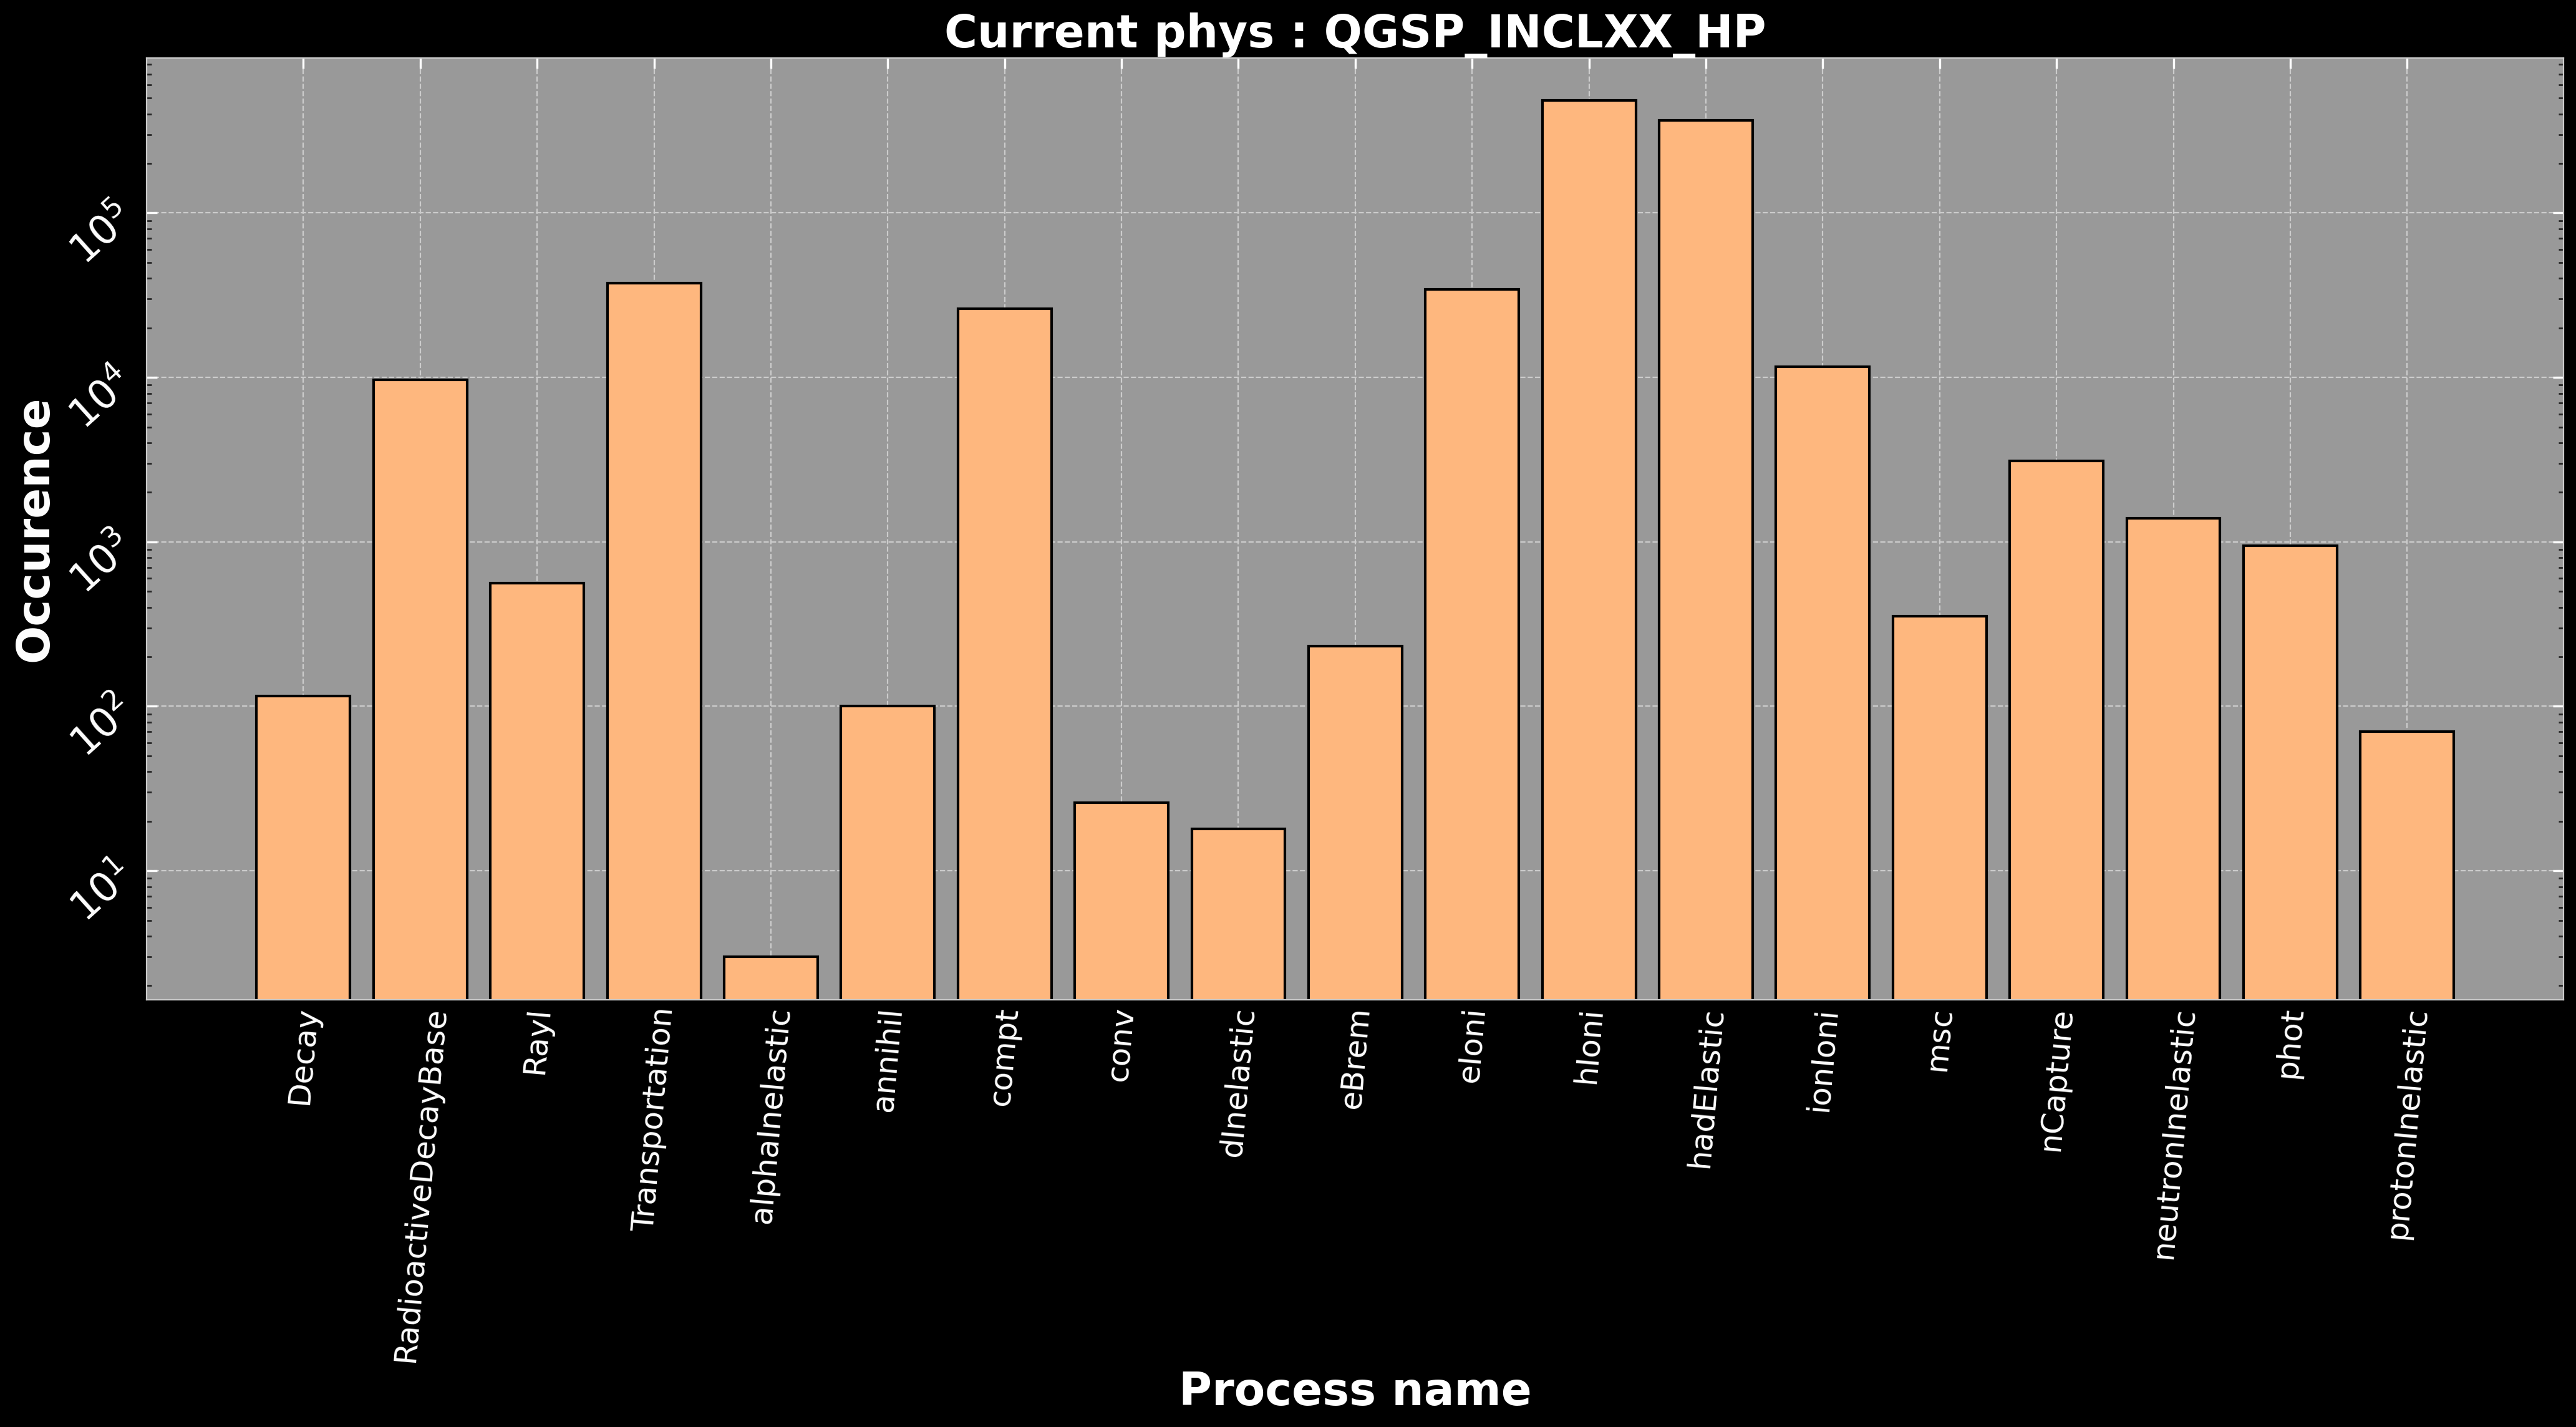
\includegraphics[width=0.95\textwidth]{{images/process_dist_E100_phQGSP_INCLXX_HP.png}}
	\captionof{figure}{}\label{fig:3}
\end{figure}
\newpage

\subsection{Process distribution in two different physics lists}
\begin{figure}[h]
	\centering
	\captionsetup{font={normalsize}}
	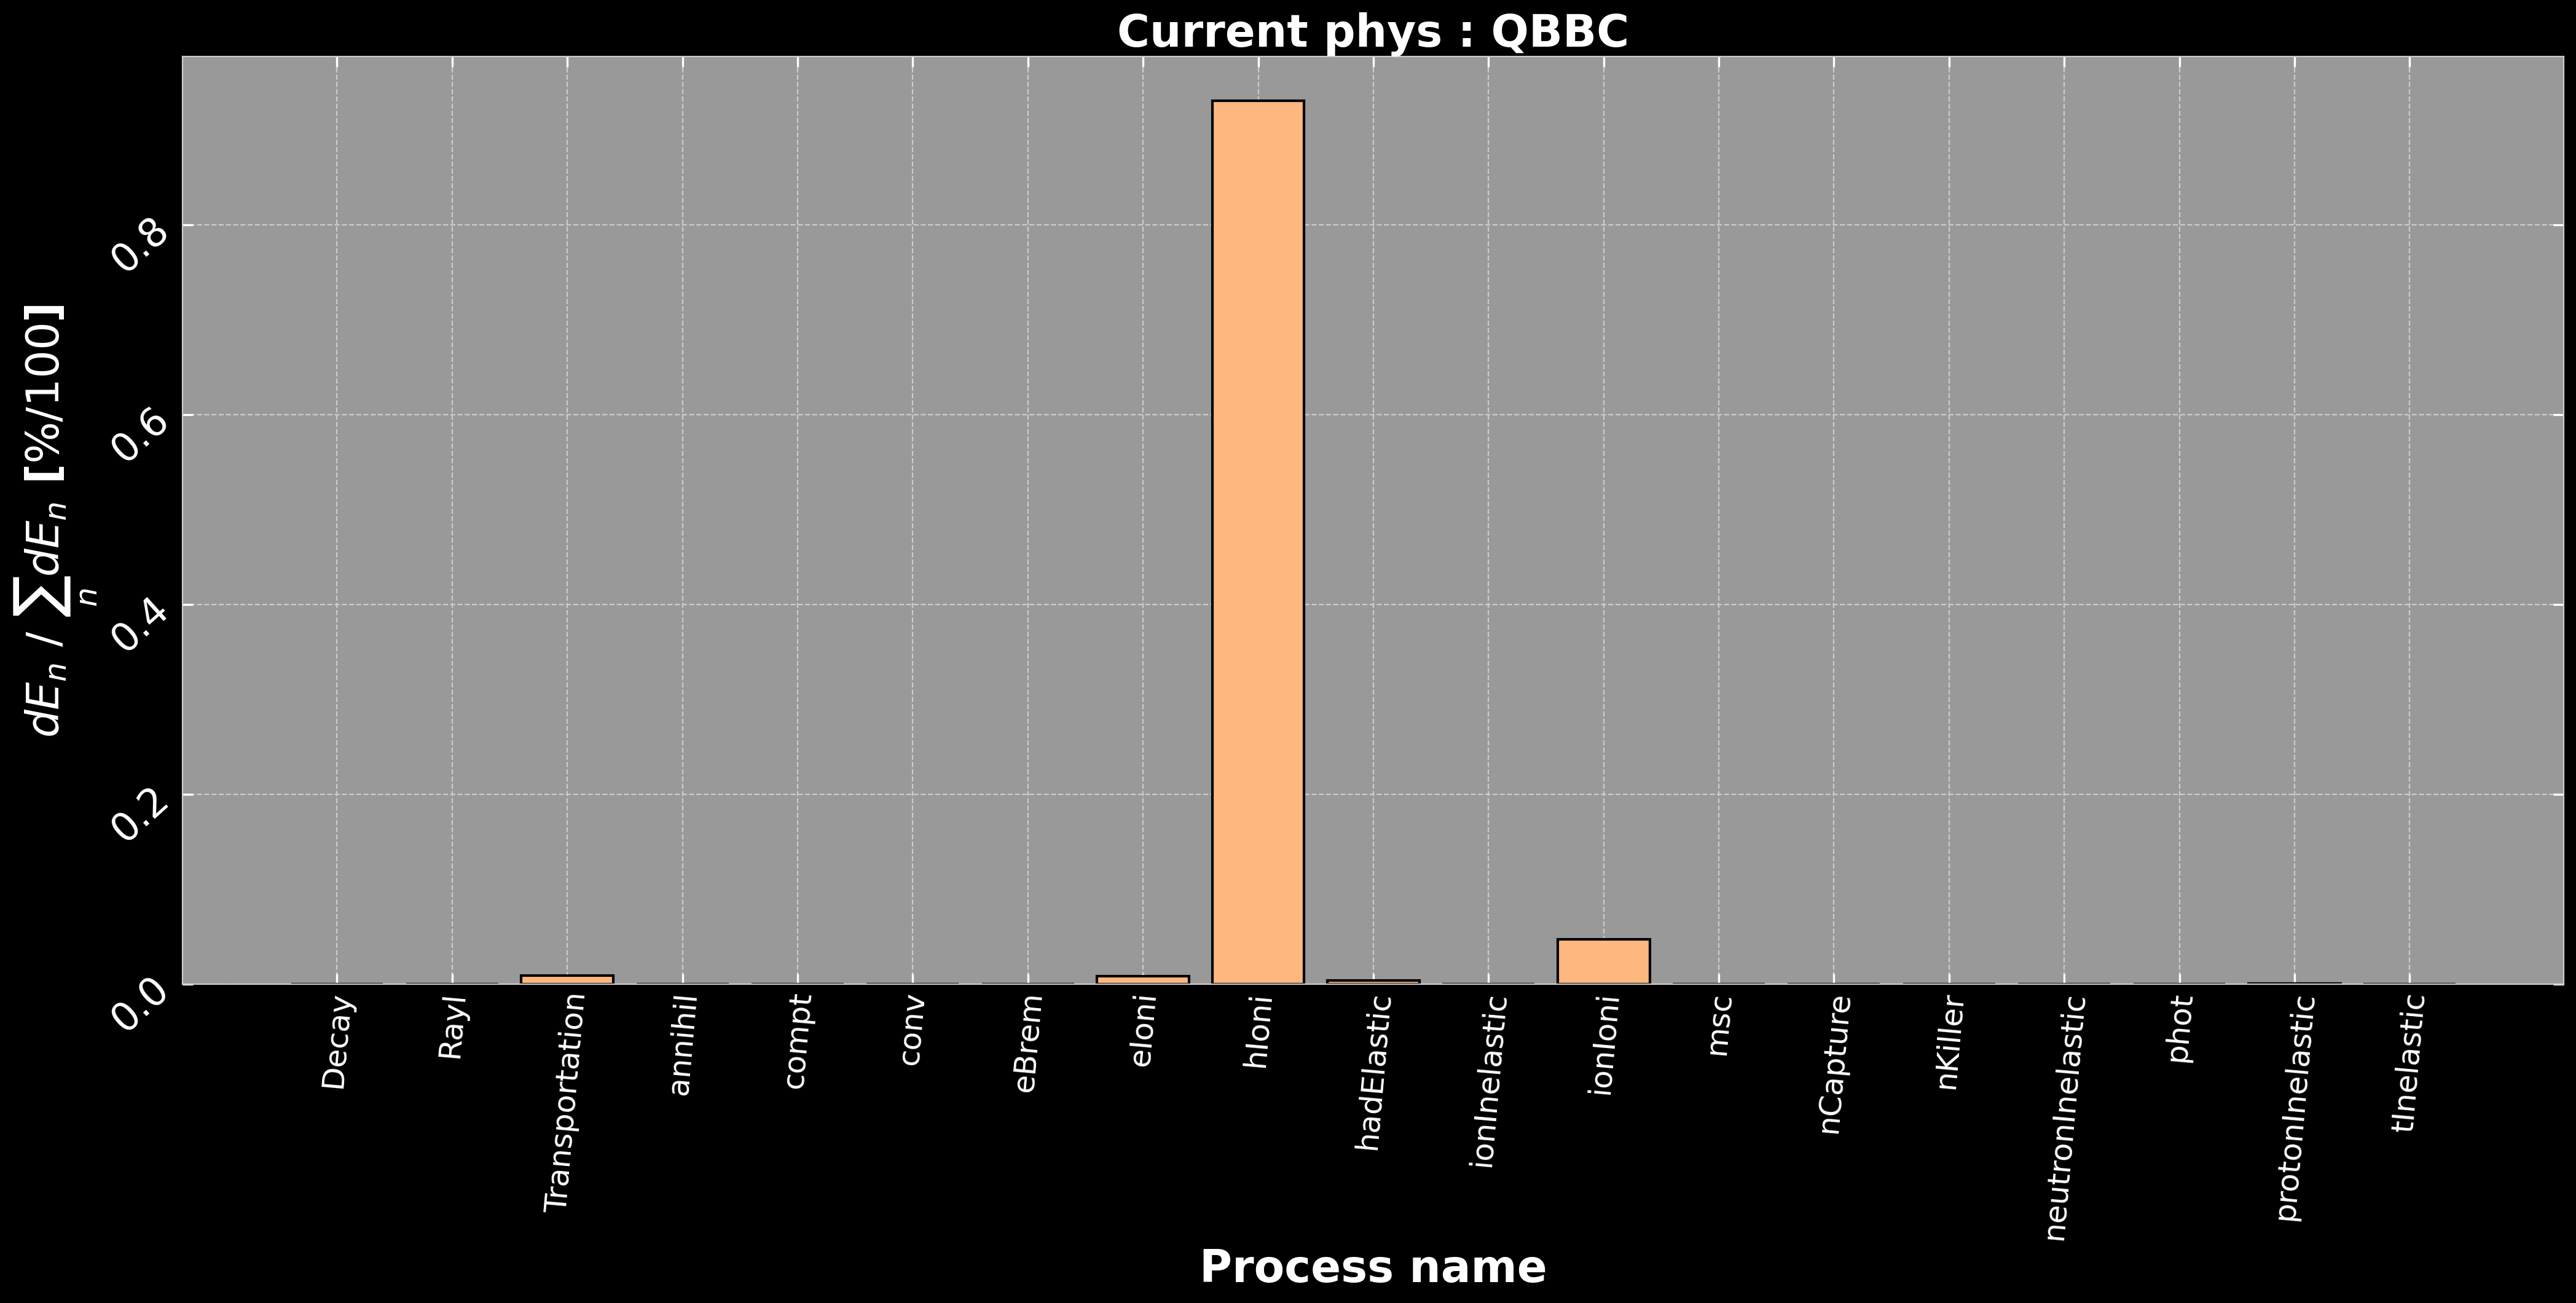
\includegraphics[width=0.95\textwidth]{{images/process_dist_weighted_E100_phQBBC.png}}
	\captionof{figure}{}\label{fig:4}
\end{figure}
\vspace{-5pt}
\begin{figure}[h]
	\centering
	\captionsetup{font={normalsize}}
	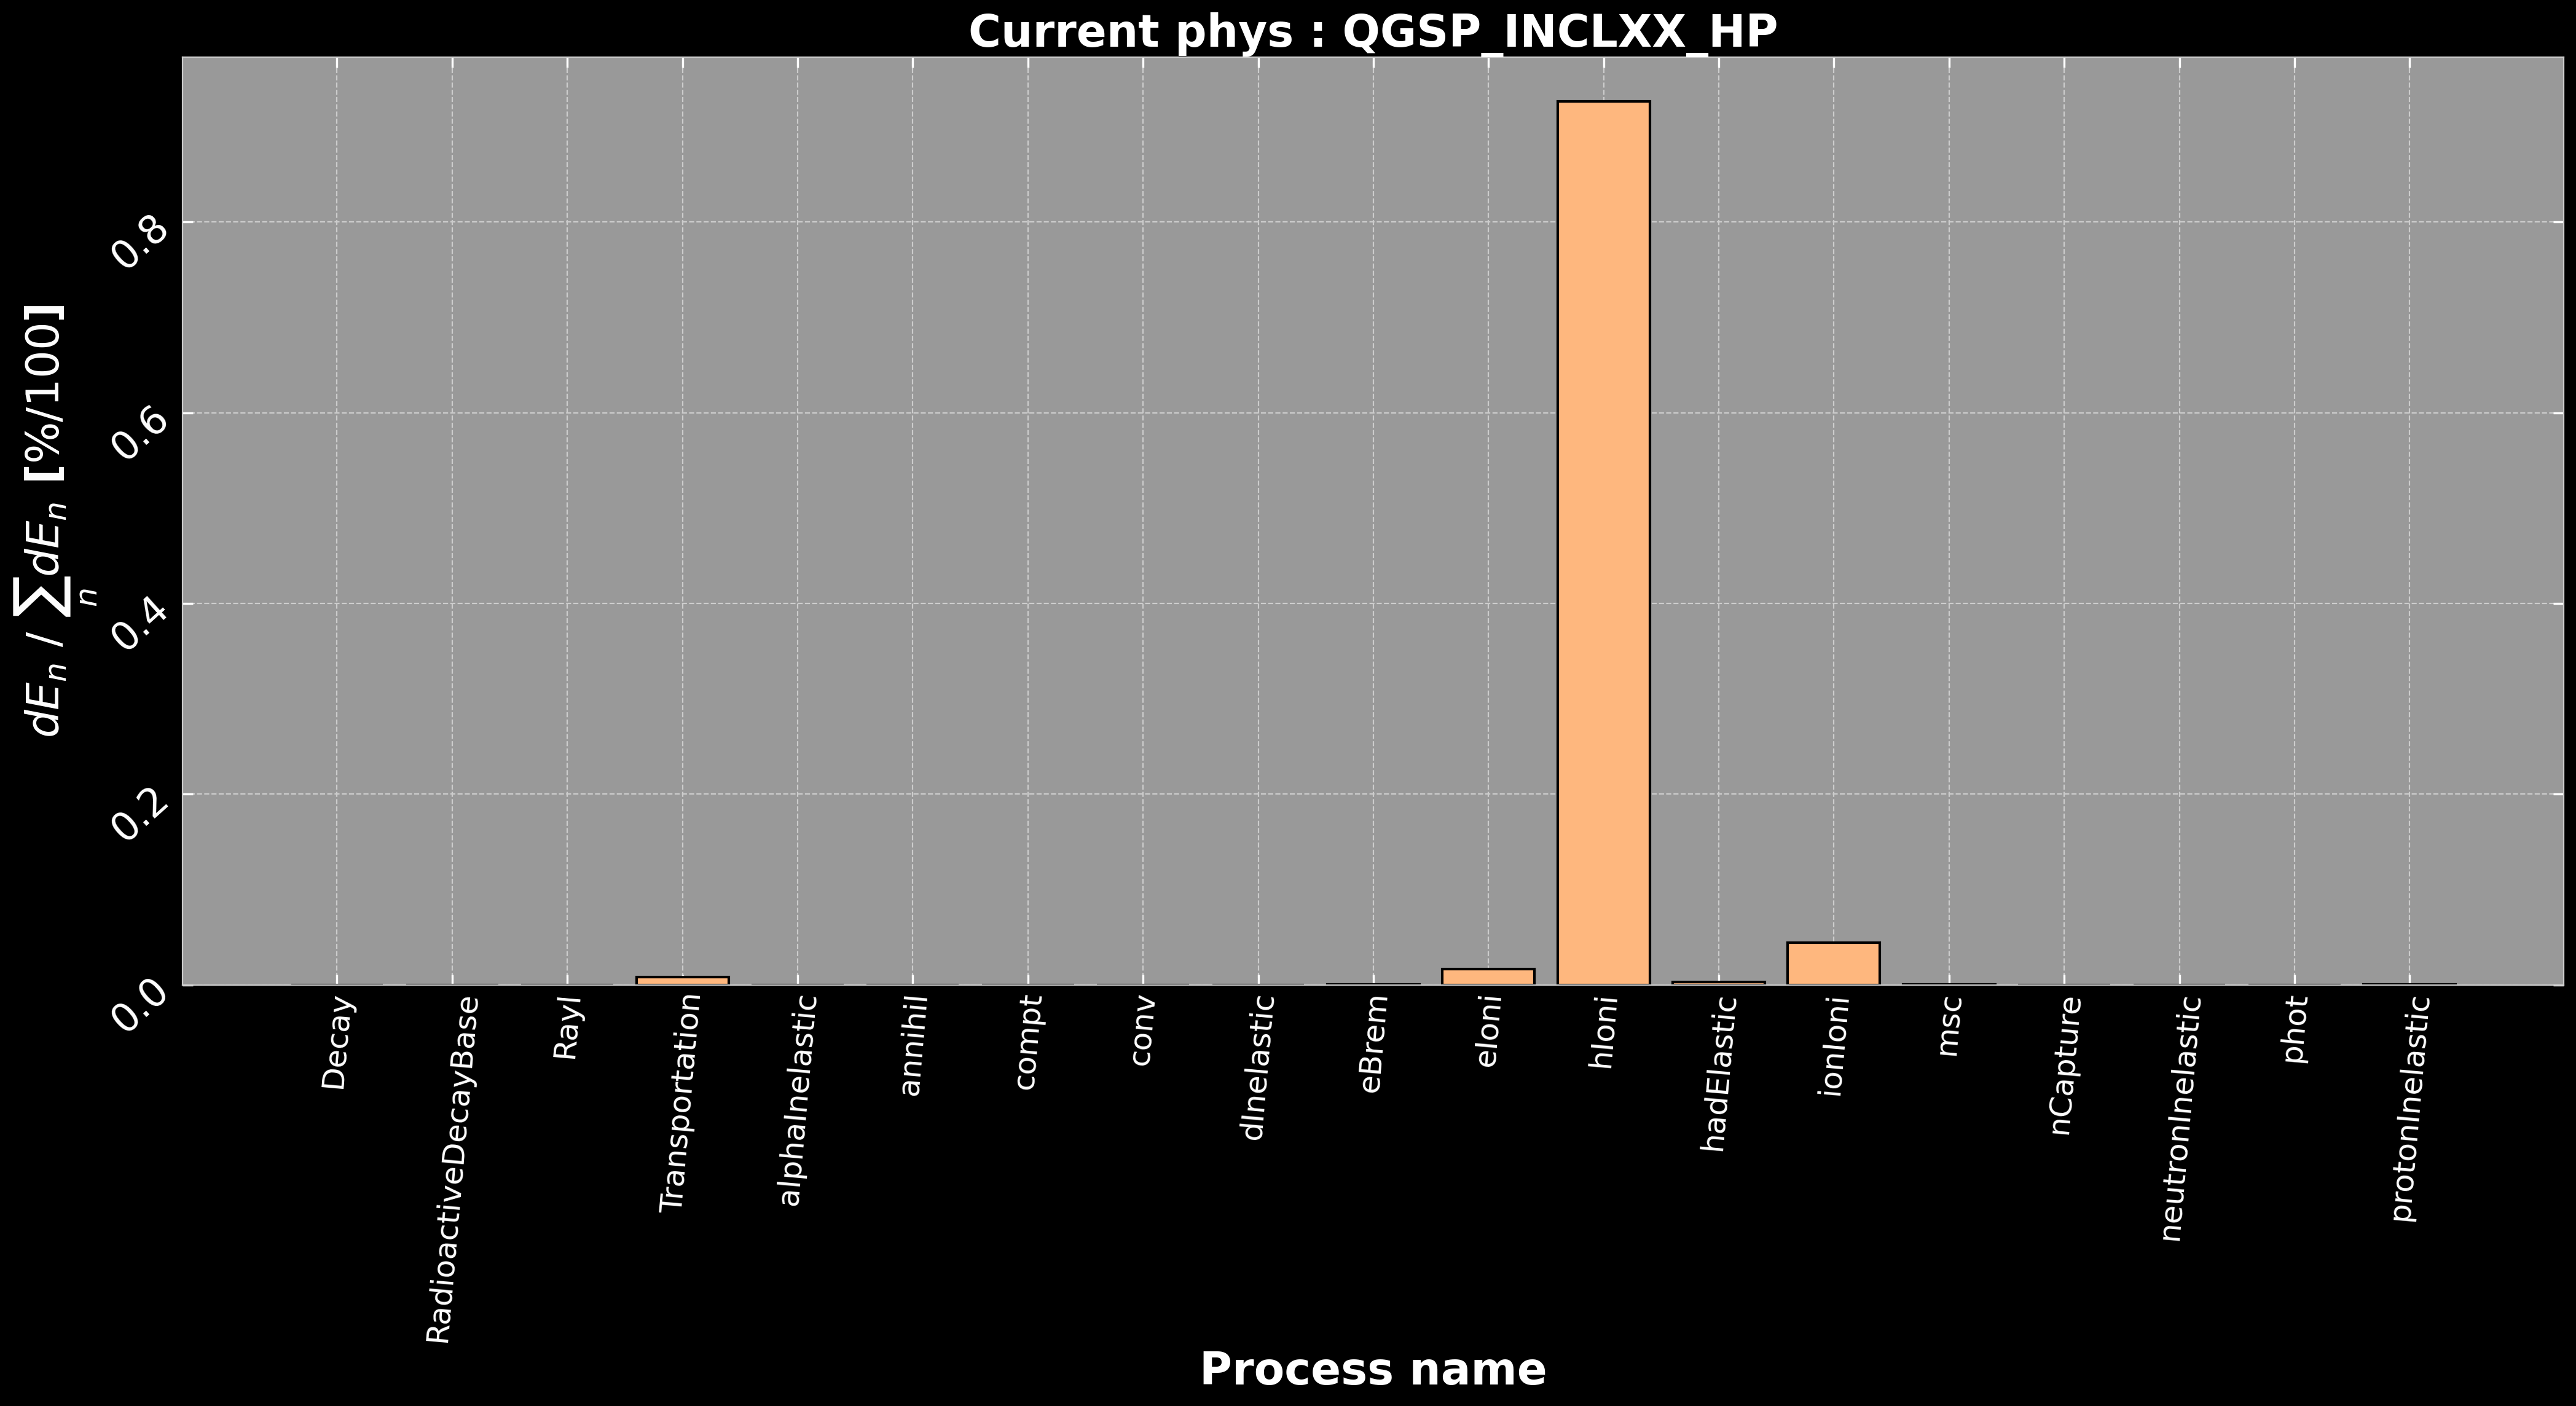
\includegraphics[width=0.95\textwidth]{{images/process_dist_weighted_E100_phQGSP_INCLXX_HP.png}}
	\captionof{figure}{}\label{fig:5}
\end{figure}
\newpage

\subsection{Particle steps during the simulation}
\begin{figure}[h]
	\centering
	\captionsetup{font={normalsize}}
	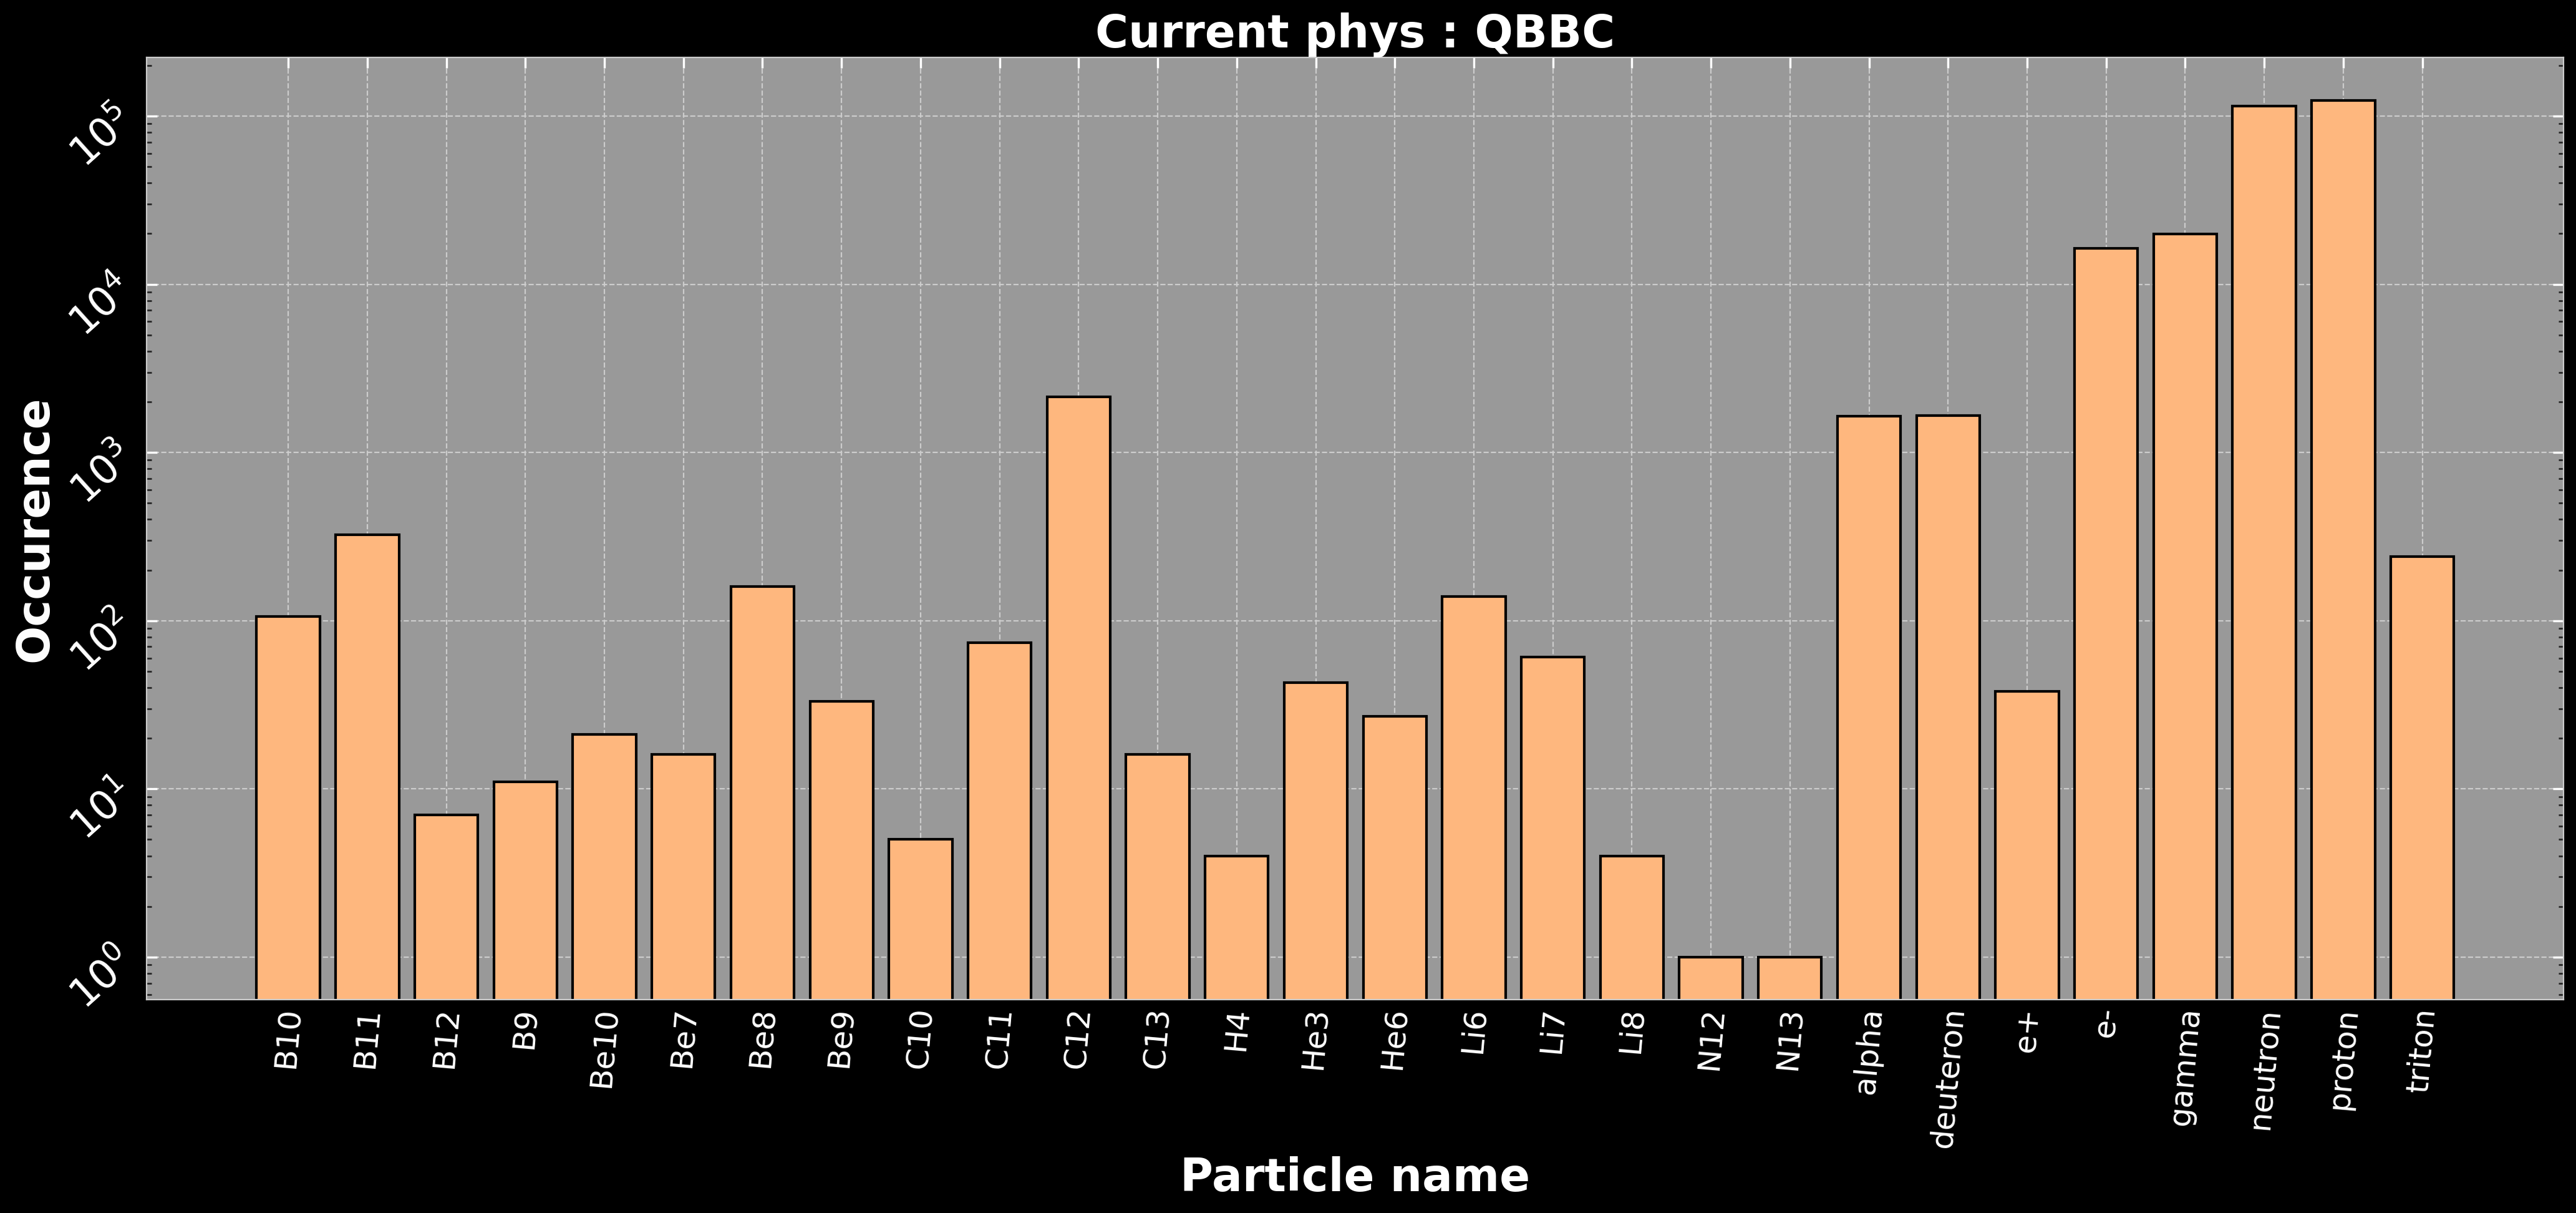
\includegraphics[width=0.95\textwidth]{{images/particle_dist_E100_phQBBC.png}}
	\captionof{figure}{}\label{fig:6}
\end{figure}
\vspace{-5pt}
\begin{figure}[h]
	\centering
	\captionsetup{font={normalsize}}
	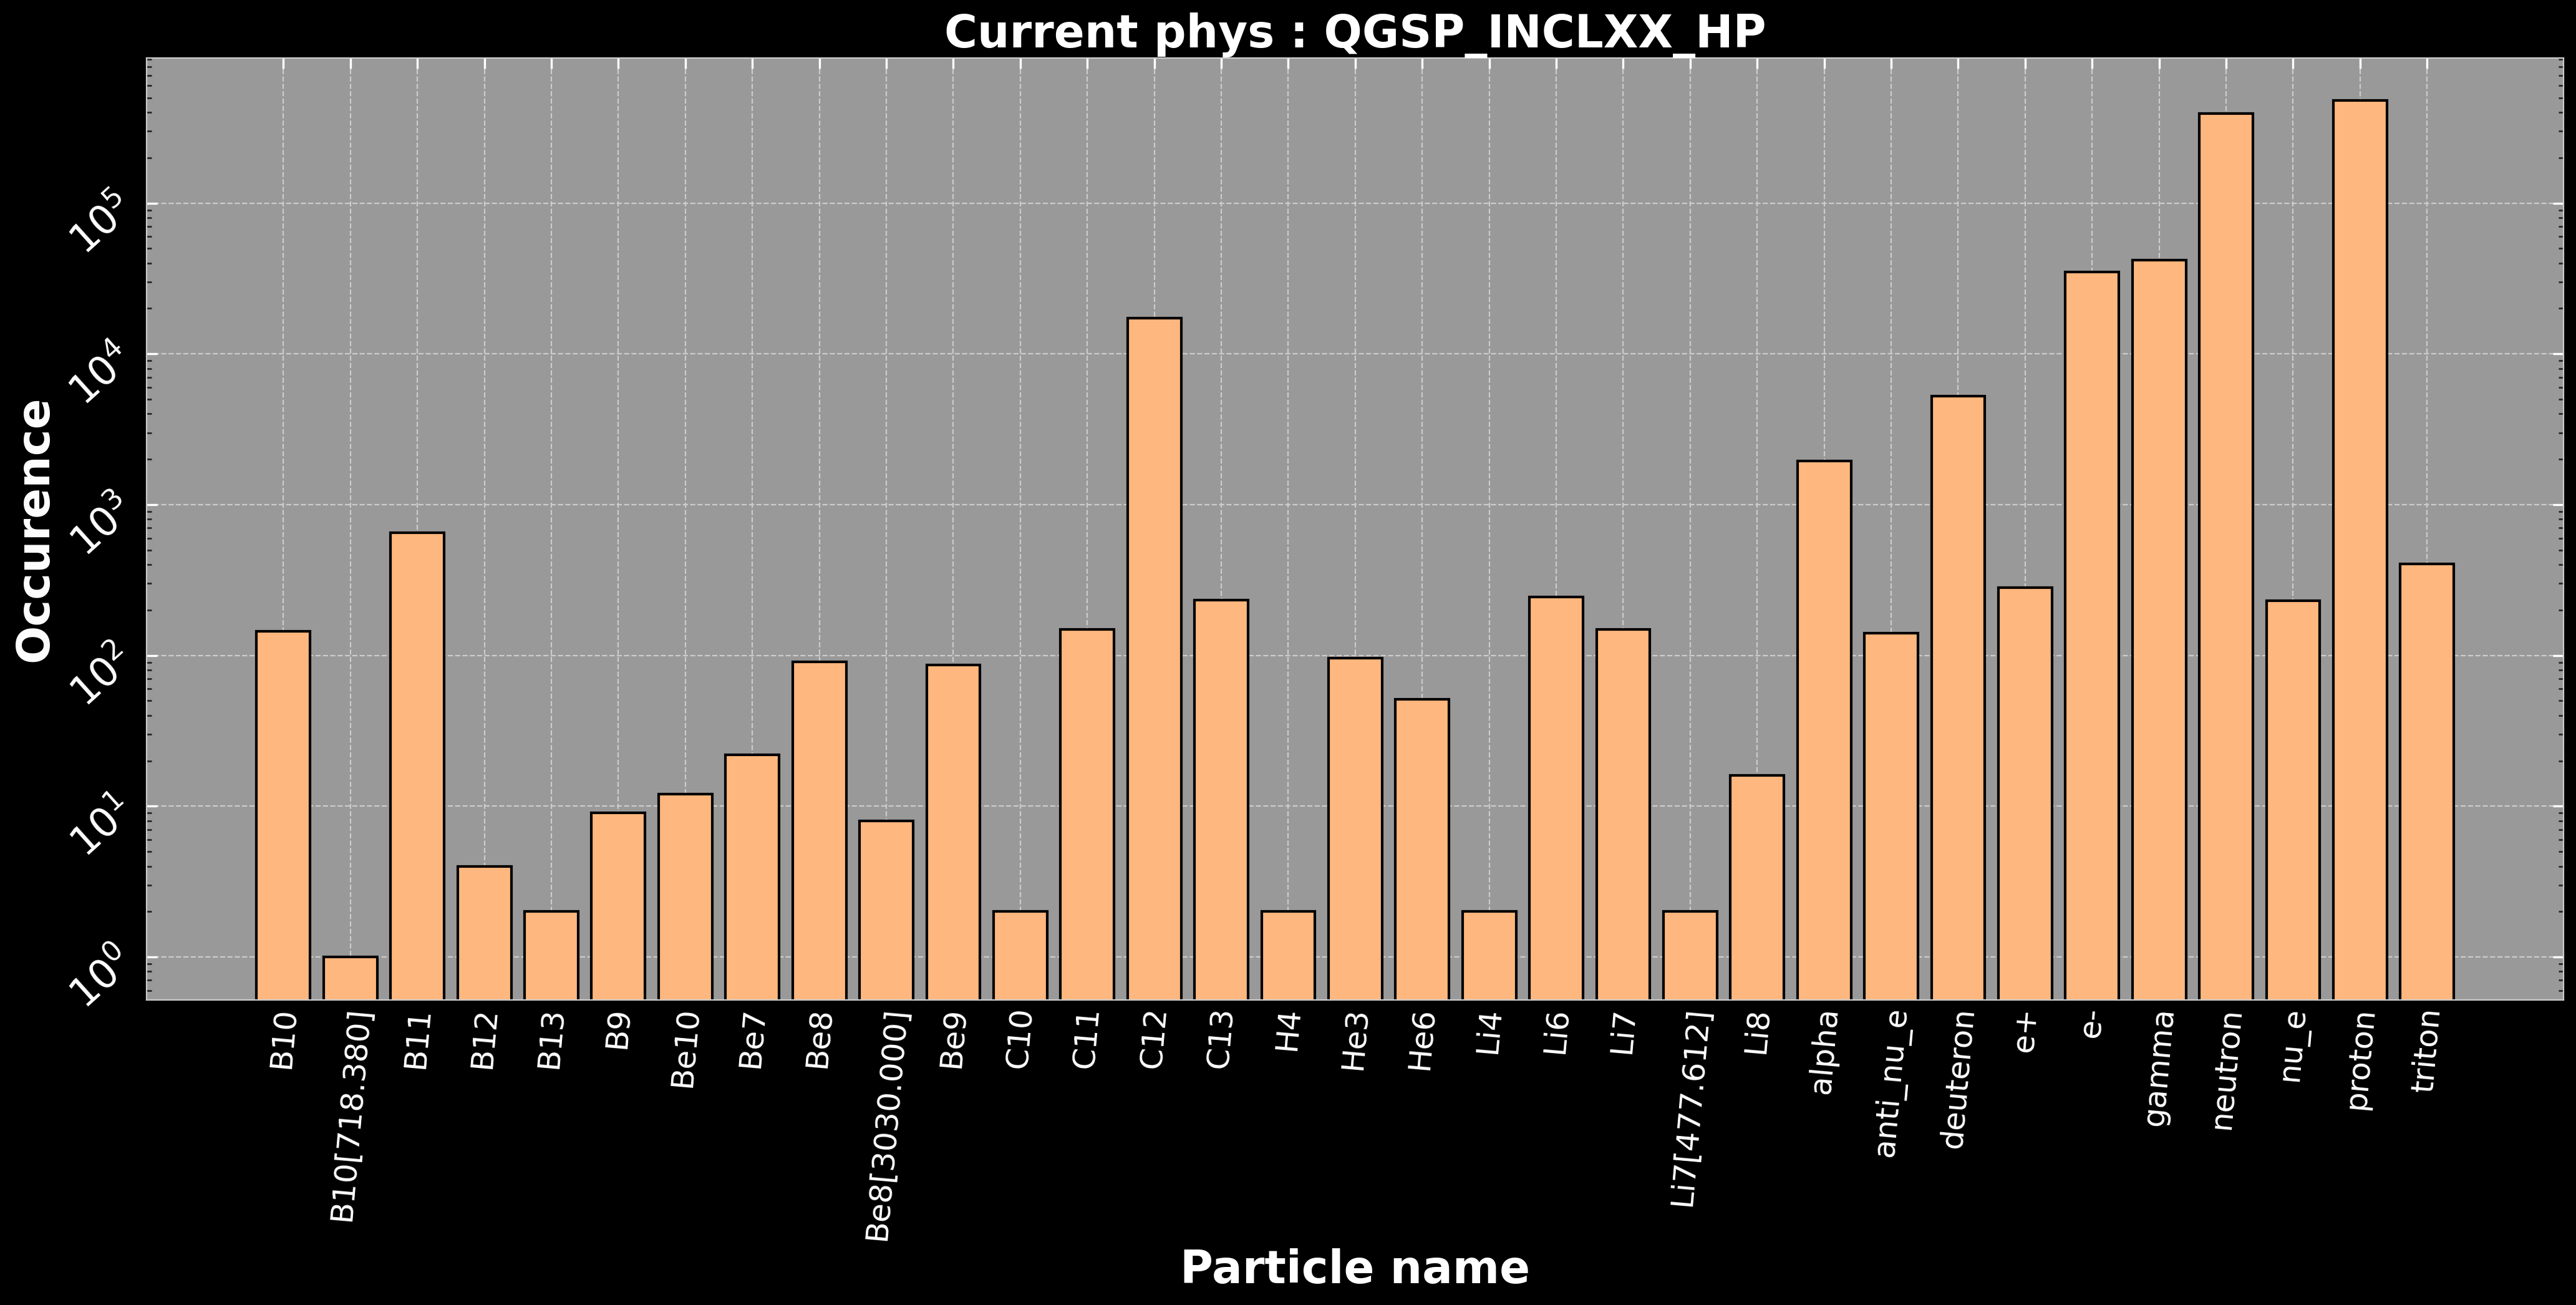
\includegraphics[width=0.95\textwidth]{{images/particle_dist_E100_phQGSP_INCLXX_HP.png}}
	\captionof{figure}{}\label{fig:7}
\end{figure}